\documentclass[spec, och, labwork]{shiza}
% параметр - тип обучения - одно из значений:
%    spec     - специальность
%    bachelor - бакалавриат (по умолчанию)
%    master   - магистратура
% параметр - форма обучения - одно из значений:
%    och   - очное (по умолчанию)
%    zaoch - заочное
% параметр - тип работы - одно из значений:
%    referat    - реферат
%    coursework - курсовая работа (по умолчанию)
%    diploma    - дипломная работа
%    pract      - отчет по практике
% параметр - включение шрифта
%    times    - включение шрифта Times New Roman (если установлен)
%               по умолчанию выключен
\usepackage{subfigure}
\usepackage{tikz,pgfplots}
\pgfplotsset{compat=1.5}
\usepackage{float}

%\usepackage{titlesec}
\setcounter{secnumdepth}{4}
%\titleformat{\paragraph}
%{\normalfont\normalsize}{\theparagraph}{1em}{}
%\titlespacing*{\paragraph}
%{35.5pt}{3.25ex plus 1ex minus .2ex}{1.5ex plus .2ex}

\titleformat{\paragraph}[block]
{\hspace{1.25cm}\normalfont}
{\theparagraph}{1ex}{}
\titlespacing{\paragraph}
{0cm}{2ex plus 1ex minus .2ex}{.4ex plus.2ex}

% --------------------------------------------------------------------------%


\usepackage[T2A]{fontenc}
\usepackage[utf8]{inputenc}
\usepackage{graphicx}
\graphicspath{ {./images/} }
\usepackage{tempora}

\usepackage[sort,compress]{cite}
\usepackage{amsmath}
\usepackage{amssymb}
\usepackage{amsthm}
\usepackage{fancyvrb}
\usepackage{listings}
\usepackage{listingsutf8}
\usepackage{longtable}
\usepackage{array}
\usepackage[english,russian]{babel}

% \usepackage[colorlinks=true]{hyperref}
\usepackage{url}

\usepackage{underscore}
\usepackage{setspace}
\usepackage{indentfirst} 
\usepackage{mathtools}
\usepackage{amsfonts}
\usepackage{enumitem}
\usepackage{tikz}
\usepackage{minted}

\newcommand{\eqdef}{\stackrel {\rm def}{=}}
\newcommand{\specialcell}[2][c]{%
\begin{tabular}[#1]{@{}c@{}}#2\end{tabular}}

\renewcommand\theFancyVerbLine{\small\arabic{FancyVerbLine}}

\newtheorem{lem}{Лемма}

\begin{document}

% Кафедра (в родительном падеже)
\chair{}

% Тема работы
\title{Счётчики}

% Курс
\course{3}

% Группа
\group{331}

% Факультет (в родительном падеже) (по умолчанию "факультета КНиИТ")
\department{факультета КНиИТ}

% Специальность/направление код - наименование
%\napravlenie{09.03.04 "--- Программная инженерия}
%\napravlenie{010500 "--- Математическое обеспечение и администрирование информационных систем}
%\napravlenie{230100 "--- Информатика и вычислительная техника}
%\napravlenie{231000 "--- Программная инженерия}
\napravlenie{100501 "--- Компьютерная безопасность}

% Для студентки. Для работы студента следующая команда не нужна.
% \studenttitle{Студентки}

% Фамилия, имя, отчество в родительном падеже
\author{автор}

% Заведующий кафедрой
% \chtitle{} % степень, звание
% \chname{}

%Научный руководитель (для реферата преподаватель проверяющий работу)
\satitle{аспирант} %должность, степень, звание
\saname{А. А. Мартышкин}

% Руководитель практики от организации (только для практики,
% для остальных типов работ не используется)
% \patitle{к.ф.-м.н.}
% \paname{С.~В.~Миронов}

% Семестр (только для практики, для остальных
% типов работ не используется)
%\term{8}

% Наименование практики (только для практики, для остальных
% типов работ не используется)
%\practtype{преддипломная}

% Продолжительность практики (количество недель) (только для практики,
% для остальных типов работ не используется)
%\duration{4}

% Даты начала и окончания практики (только для практики, для остальных
% типов работ не используется)
%\practStart{30.04.2019}
%\practFinish{27.05.2019}

% Год выполнения отчета
\date{2022}

\maketitle

% Включение нумерации рисунков, формул и таблиц по разделам
% (по умолчанию - нумерация сквозная)
% (допускается оба вида нумерации)
% \secNumbering

%-------------------------------------------------------------------------------------------

\section*{Цель работы:}

Ознакомление с устройством и функционированием счётчиков и испытание синхронного
суммирующего, реверсивного и десятичного счётчиков.

\subsection*{Задание 1.}

Построим схему синхронного двоичного счётчика.

\begin{figure}[H]
    \centering
    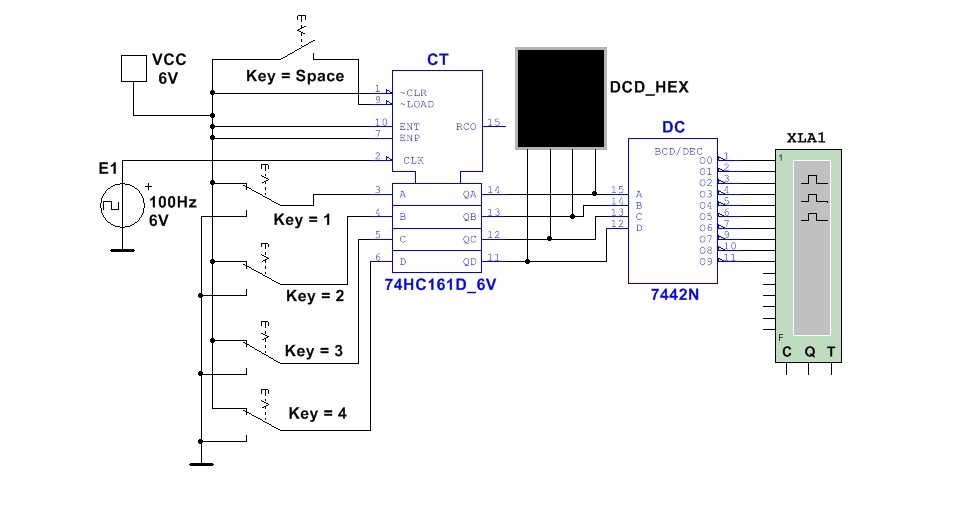
\includegraphics[width=5.28607in,height=3.2197in]{image1.jpeg}
\end{figure}

Рассмотрим схему при разомкнутом ключе Space.

\begin{figure}[H]
    \centering
    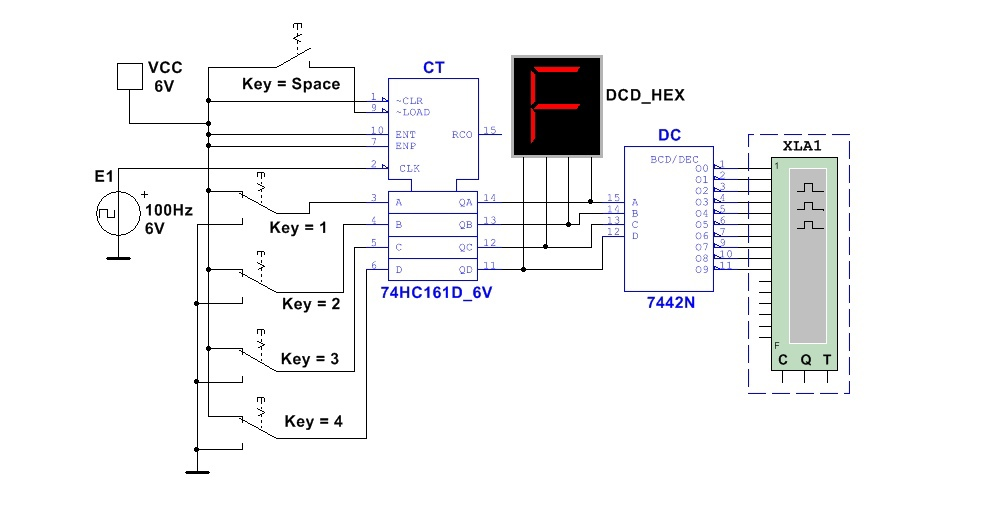
\includegraphics[width=5.6577in,height=3.37083in]{image2.jpeg}
\end{figure}

\begin{figure}[H]
    \centering
    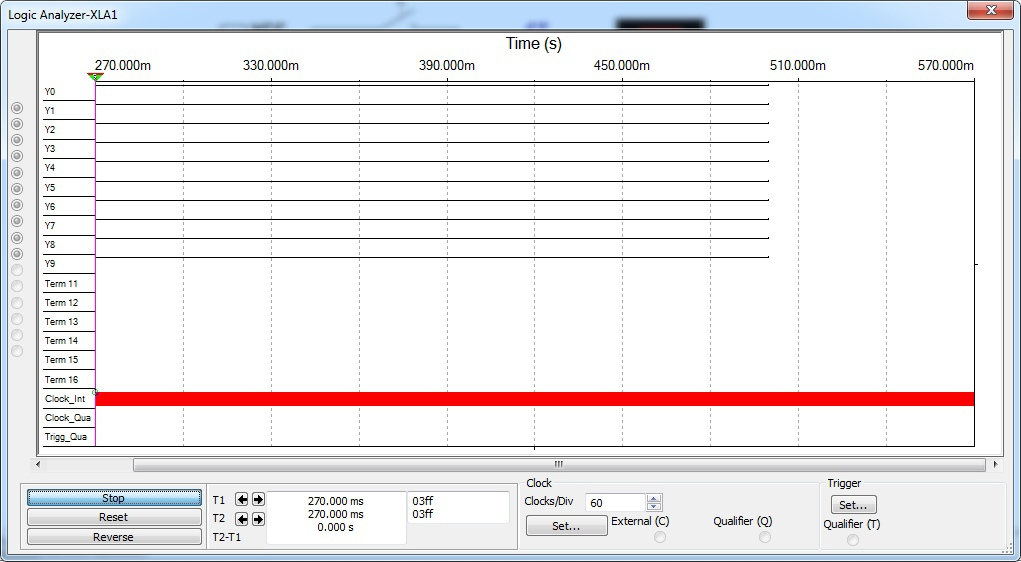
\includegraphics[width=5.83937in,height=3.21212in]{image3.jpeg}
\end{figure}

При замкнутом ключе схема выдает шестнадцатеричные цифры
в последовательности от 0 до $F$.

\begin{figure}[H]
    \centering
    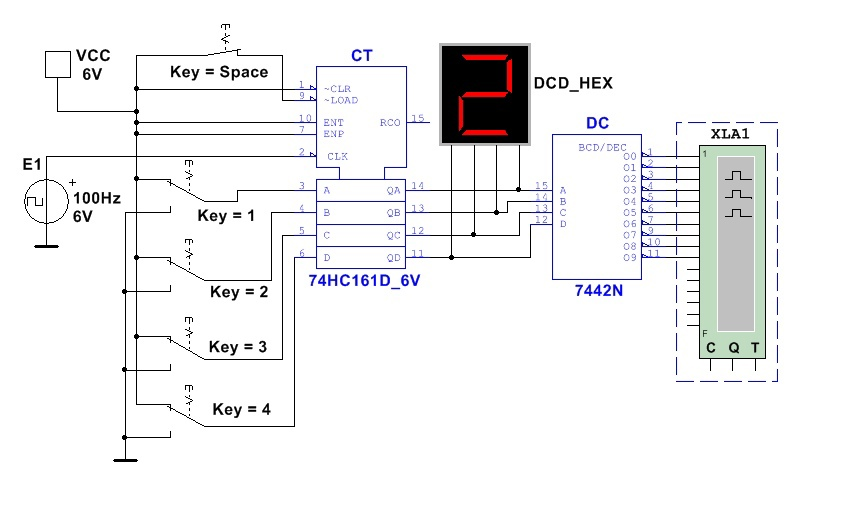
\includegraphics[width=5.68277in,height=3.42424in]{image4.jpeg}
\end{figure}

\begin{figure}[H]
    \centering
    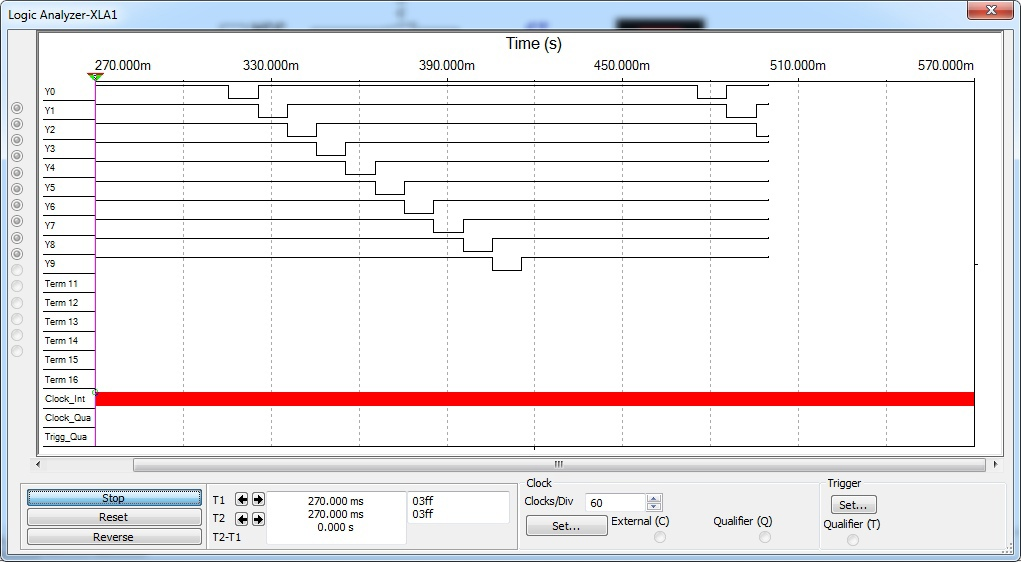
\includegraphics[width=5.64656in,height=3.10606in]{image5.jpeg}
\end{figure}


\subsection*{Задание 2.}

При установке ключей в различные положения, получим последовательность 0
и 1 на экране.

\begin{figure}[H]
    \centering
    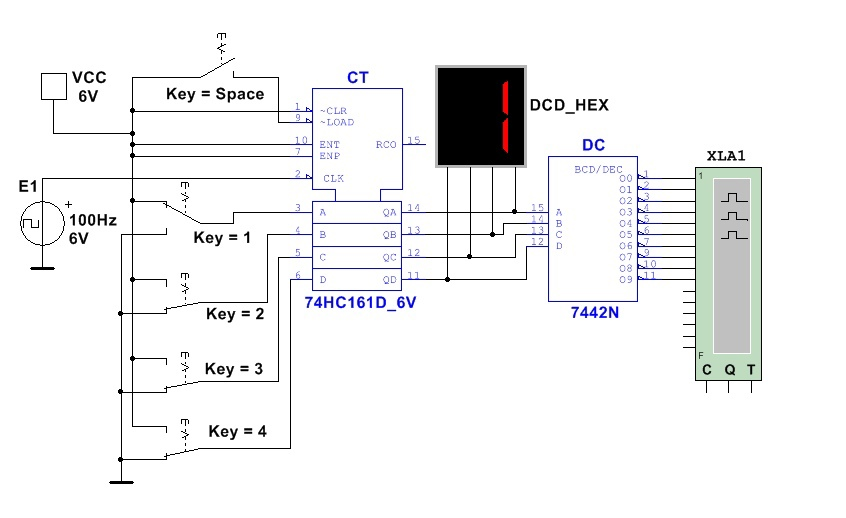
\includegraphics[width=5.29307in,height=3.24242in]{image6.jpeg}
\end{figure}

\begin{figure}[H]
    \centering
    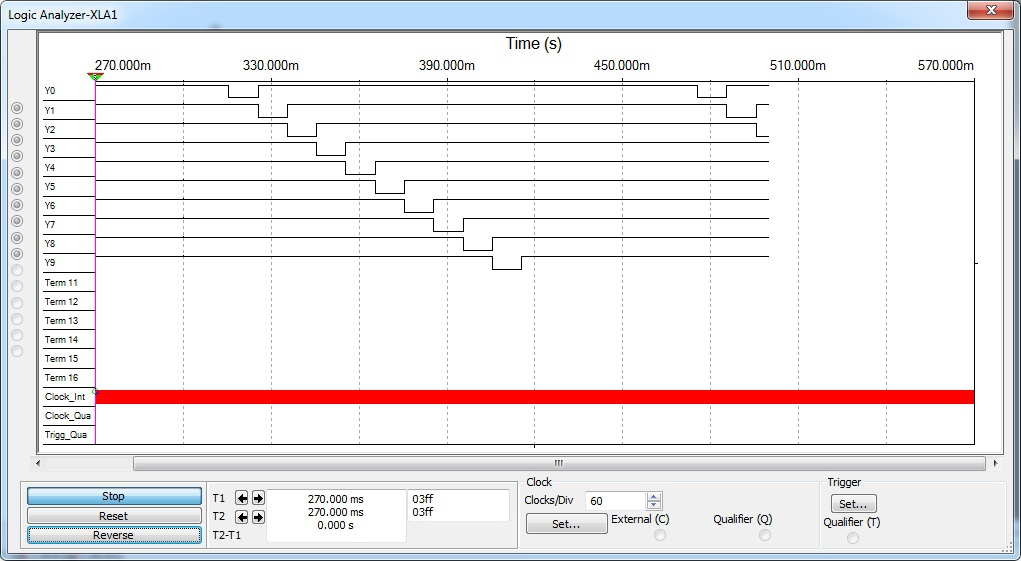
\includegraphics[width=5.74147in,height=3.15152in]{image7.jpeg}
\end{figure}


\subsection*{Задание 3.}

Построим схему реверсивного двоичного счётчика.

\begin{figure}[H]
    \centering
    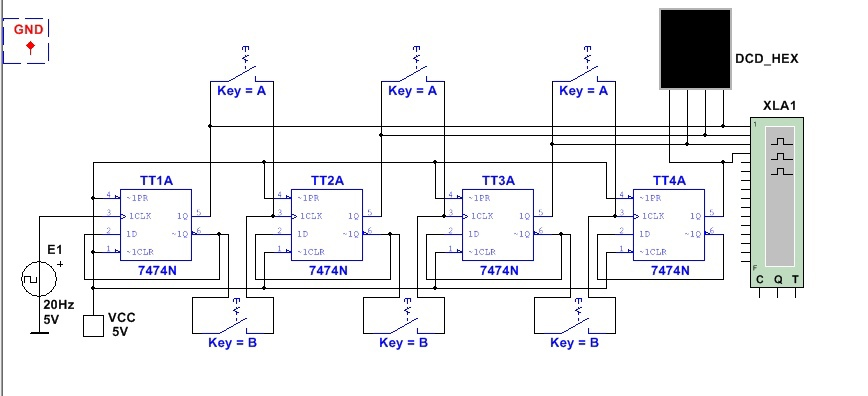
\includegraphics[width=6.11603in,height=2.81061in]{image8.jpeg}
\end{figure}

При замыкании ключей А и размыкании ключей В наблюдаем последовательное
изображение шестнадцатеричных чисел на экране в обратном порядке (от F до 0).

\begin{figure}[H]
    \centering
    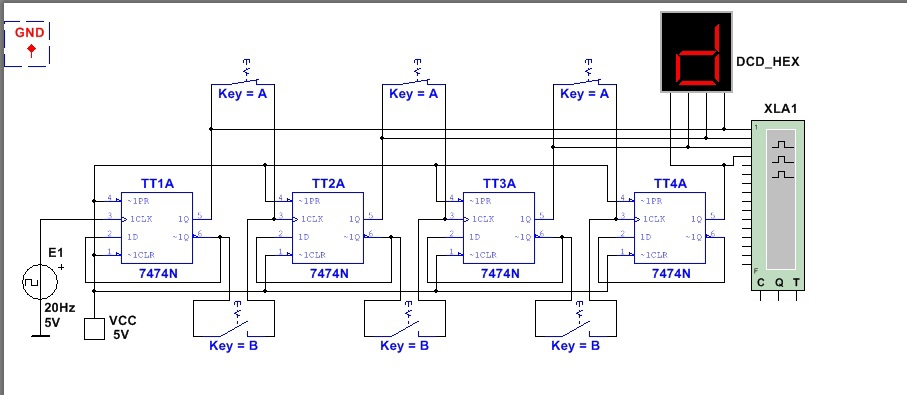
\includegraphics[width=6.45865in,height=2.79406in]{image9.jpeg}
\end{figure}

Введем указанные данные, получим следующий результат:

\begin{figure}[H]
    \centering
    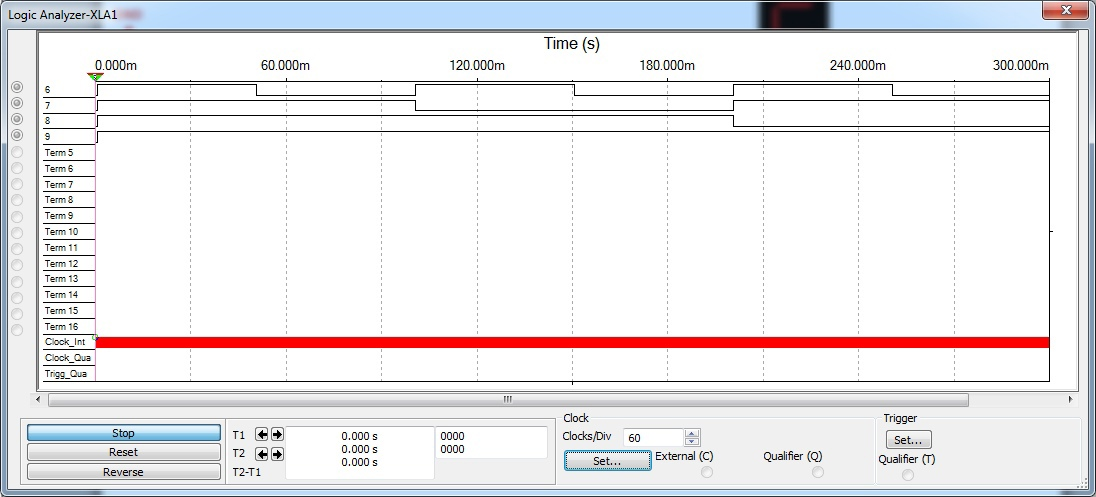
\includegraphics[width=6.04692in,height=2.73485in]{image10.jpeg}
\end{figure}

Рассмотрим обратную ситуацию с ключами.

\begin{figure}[H]
    \centering
    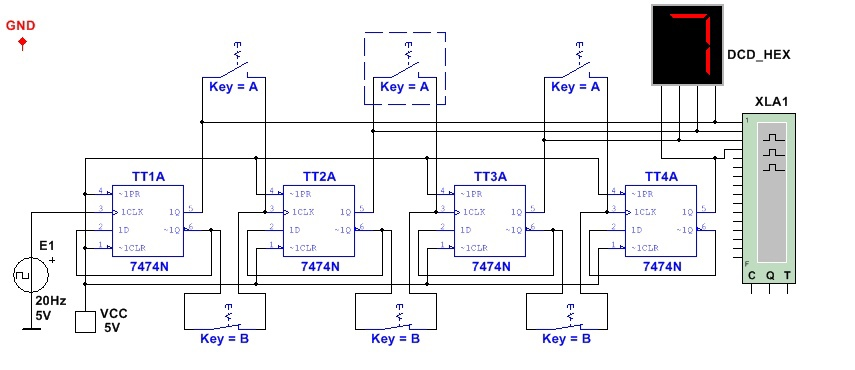
\includegraphics[width=5.56762in,height=2.41667in]{image11.jpeg}
\end{figure}

\begin{figure}[H]
    \centering
    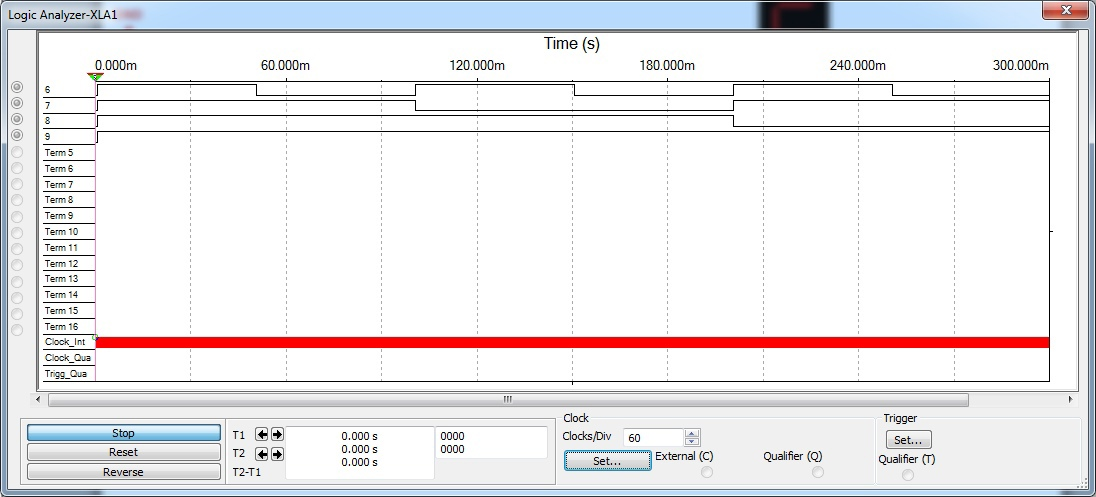
\includegraphics[width=6.19767in,height=2.80303in]{image10.jpeg}
\end{figure}


\subsection*{Задание 4.}

Построим схему десятичного счётчика.

\begin{figure}[H]
    \centering
    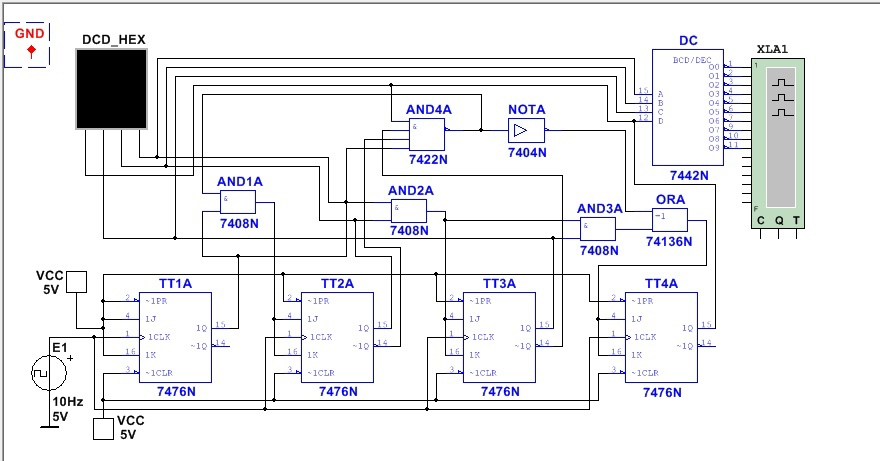
\includegraphics[width=6.45829in,height=3.3613in]{image12.jpeg}
\end{figure}

Запустим программу и в окне анализатора получим следующие результаты
моделирования.

\begin{figure}[H]
    \centering
    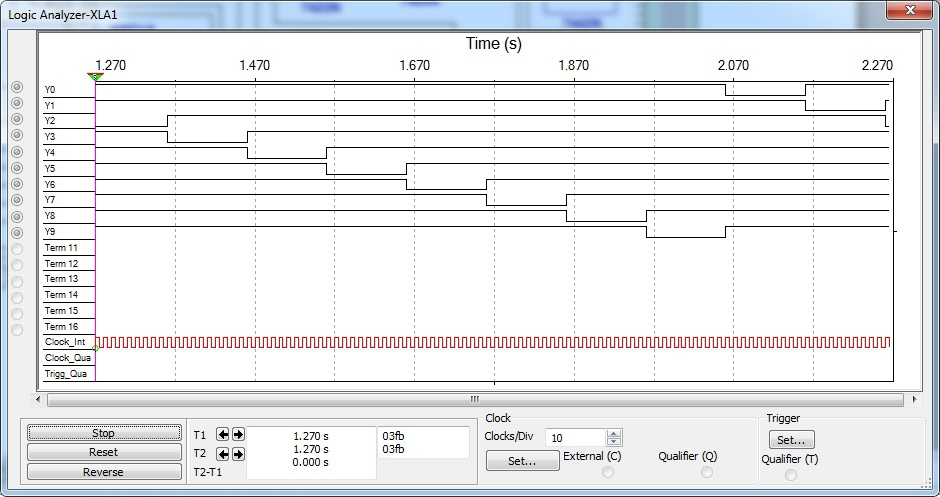
\includegraphics[width=5.56253in,height=2.94697in]{image13.jpeg}
\end{figure}

\textbf{Вывод:} ознакомились с устройством и функционированием счётчиков
и испытали синхронный суммирующий, реверсивный и десятеричный счётчики.


\section*{Тестовые задание к работе 34}

\begin{enumerate}
    \item
        \textit{Укажите, \textbf{в каком виде} фиксируется в счетчике число
        поступивших на его входи импульсов}:

        в виде двоичного кода, хранящегося в триггерах;
    
    \item
        \textit{Укажите необходимое \textbf{число выходов} двоичного счетчика
        для выдачи результатов счета 28 импульсов}:

        4;

    \item
        \textit{Укажите, в \textbf{какой момент} 5"=разрядный двоичный счетчик
        возвращается в начальное состояние}:

        при подаче на вход 32"=го импульса;

    \item
        \textit{На 7-сегментном индикаторе десятичного счетчика высвечивается
        число 5. Укажите, какое \textbf{число} будет высвечиваться на индикаторе
        при подаче на вход еще шести импульсов}:

        3;
    
    \item
        \textit{Укажите, \textbf{каким путем передаются сигналы} от разряда к
        разряду в синхронном счетчике}:

        посредством специальной переключающей схемы;

    \item
        \textit{Укажите, что понимают под \textbf{коэффициентом пересчета}
        счетчика}:

        это модуль счета, характеризуемый числом устойчивых состояний счетчика;

    \item
        \textit{Укажите, чему равен \textbf{модуль $M$ пересчета} двоичного 
        $n$"=разрядного счетчика:}

        $M = 2^n$;

    \item
        \textit{Укажите, сколько \textbf{триггеров} должен иметь 
        двоично"=кодированный счетчик с коэффициентом пересчета $M = 8$}:

        3;
    
    \item
        \textit{Укажите \textbf{пути и средства}, с помощью которых изменяется
        направление счета в реверсивном счетчике}:

        направление счета изменяется путем изменения вида межразрядных связей.
\end{enumerate}

\end{document}
